%%
%% Copyright 2007, 2008, 2009 Elsevier Ltd
%%
%% This file is part of the 'Elsarticle Bundle'.
%% ---------------------------------------------
%%
%% It may be distributed under the conditions of the LaTeX Project Public
%% License, either version 1.2 of this license or (at your option) any
%% later version.  The latest version of this license is in
%%    http://www.latex-project.org/lppl.txt
%% and version 1.2 or later is part of all distributions of LaTeX
%% version 1999/12/01 or later.
%%
%% The list of all files belonging to the 'Elsarticle Bundle' is
%% given in the file `manifest.txt'.
%%

%% Template article for Elsevier's document class `elsarticle'
%% with numbered style bibliographic references
%% SP 2008/03/01
%%
%%
%%
%% $Id: elsarticle-template-num.tex 4 2009-10-24 08:22:58Z rishi $
%%
%%
\documentclass[final,5p,times]{elsarticle}

%% Use the option review to obtain double line spacing
%% \documentclass[preprint,review,12pt]{elsarticle}

%% Use the options 1p,twocolumn; 3p; 3p,twocolumn; 5p; or 5p,twocolumn
%% for a journal layout:
%% \documentclass[final,1p,times]{elsarticle}
%% \documentclass[final,1p,times,twocolumn]{elsarticle}
%% \documentclass[final,3p,times]{elsarticle}
%% \documentclass[final,3p,times,twocolumn]{elsarticle}
%% \documentclass[final,5p,times]{elsarticle}
%% \documentclass[final,5p,times,twocolumn]{elsarticle}

%% if you use PostScript figures in your article
%% use the graphics package for simple commands
%% \usepackage{graphics}
%% or use the graphicx package for more complicated commands
%% \usepackage{graphicx}
%% or use the epsfig package if you prefer to use the old commands
%% \usepackage{epsfig}
\usepackage{todonotes}
%% The amssymb package provides various useful mathematical symbols
\usepackage{amssymb}
%% The amsthm package provides extended theorem environments
%% \usepackage{amsthm}

%% The lineno packages adds line numbers. Start line numbering with
%% \begin{linenumbers}, end it with \end{linenumbers}. Or switch it on
%% for the whole article with \linenumbers after \end{frontmatter}.
%% \usepackage{lineno}

%% natbib.sty is loaded by default. However, natbib options can be
%% provided with \biboptions{...} command. Following options are
%% valid:

%%   round  -  round parentheses are used (default)
%%   square -  square brackets are used   [option]
%%   curly  -  curly braces are used      {option}
%%   angle  -  angle brackets are used    <option>
%%   semicolon  -  multiple citations separated by semi-colon
%%   colon  - same as semicolon, an earlier confusion
%%   comma  -  separated by comma
%%   numbers-  selects numerical citations
%%   super  -  numerical citations as superscripts
%%   sort   -  sorts multiple citations according to order in ref. list
%%   sort&compress   -  like sort, but also compresses numerical citations
%%   compress - compresses without sorting
%%
%% \biboptions{comma,round}

% \biboptions{}


\begin{document}

\begin{frontmatter}

%% Title, authors and addresses

%% use the tnoteref command within \title for footnotes;
%% use the tnotetext command for the associated footnote;
%% use the fnref command within \author or \address for footnotes;
%% use the fntext command for the associated footnote;
%% use the corref command within \author for corresponding author footnotes;
%% use the cortext command for the associated footnote;
%% use the ead command for the email address,
%% and the form \ead[url] for the home page:
%%
%% \title{Title\tnoteref{label1}}
%% \tnotetext[label1]{}
%% \author{Name\corref{cor1}\fnref{label2}}
%% \ead{email address}
%% \ead[url]{home page}
%% \fntext[label2]{}
%% \cortext[cor1]{}
%% \address{Address\fnref{label3}}
%% \fntext[label3]{}

\title{CAP in practice: HBase}

%% use optional labels to link authors explicitly to addresses:
%% \author[label1,label2]{<author name>}
%% \address[label1]{<address>}
%% \address[label2]{<address>}

\author{Thomas Uyttendaele}

\address{}

\begin{abstract}
%% Text of abstract

\end{abstract}

\begin{keyword}
%% keywords here, in the form: keyword \sep keyword
%% MSC codes here, in the form: \MSC code \sep code
%% or \MSC[2008] code \sep code (2000 is the default)

\end{keyword}

\end{frontmatter}

%%
%% Start line numbering here if you want
%%
% \linenumbers

%% main text
\section{Introduction}

New online services, more online users means more data, data and load a single server can't handle. More and more database systems are distributed, for higher availability in case of an unexpected crash but also for horizontal distribution: the data of a single database is spread over different systems. These new services have also different requirements, an update doesn't need to be visible for all users immediately, it can take time and the concept eventual consistency was there. 

Over the past years, many new systems have been build on this wave of changes, and they are categorized under NoSQL. But some applications have a lot of data, the need to have the consistent data and being able to work in a highly distributed environment, called CP systems in the CAP Theorem. Two examples that offer these guarantees are HBase and MongoDB. They greatly differ in supported queries on their system, but what happens if you only use the bare essentials and compare their behaviour in a distributed environment going from expected shut downs of instances towards crashes and network partitions. 

In this article, a comparison of both this systems on these 3 behaviours will be made. In chapter \ref{sec:CAPTheorem} a brief overview of the CAP Theorem is given, chapter \ref{sec:hbaseandmongodb} discusses HBase and MongoDB on paper. Chapter \ref{sec:testmethod} gives an overview of the used test method and chapter \ref{sec:result} presents the results. To end in chapter \ref{sec:futurework} future work is presented, an overview of related work is given in chapter \ref{sec:related work} and a conclusion is made in chapter \ref{sec:conclusion}.  

\section{The CAP Theorem\cite{brewer2000towards}\cite{brewer2012cap}}\label{sec:CAPTheorem}
The CAP Theorem was introduced by E. Brewer \cite{brewer2000towards}  in 2000 and discusses 3 properties of which each network shared-data system can guarantee at most 2: (definitions based on \cite{brewer2012cap})
\begin{itemize}
\item (Strict)\textbf{C}onsistency: The system acts like there is only single storage 
\item High \textbf{a}vailability: The system is available (for updates)
\item \textbf{P}artition tolerance: A split in the network let the different partitions still act as a single system. 
\end{itemize}
Designers used this model to explain their design decisions, others used it to compare different system but sometimes it was misused. As E. Brewer explains 12 year after the launch, the "2 of 3" can be misleading.

One of the reasons is that there exist several types of consistency, partition tolerance and different availability guarantees. These choices need to be made several times in the different subsystems and the end solution is not black or white. 

At first glance, it also looks like partition tolerance has to be implemented and therefore consistency and availability needs to be given up. In the practice, partition splits are only rare and therefore both consistency and availability can be allowed most of the time. 

Each of the 3 choices will be discussed in more detail, how their implementation could work, what the influences are and some examples. 

\subsection{CA}
When forfeiting partition tolerance, these systems provide all the time consistent data available to all nodes, except when there are one or more nodes unavailable. In that case, write requests will be not allowed. 

These systems can be build around the 2 phase commit and have cache invalidation protocols. Examples of this types are the typical relational databases roll out in clusters. 

\subsection{CP}
A consistent system with partition tolerance will provide all the time the last data, even in the case of network splits. This comes with the loss of all nodes available all the time. 

The system will allow operations only on the majority partition. In case multiple splits are present and no partition has a majority of nodes, the whole system can be unavailable. These systems can be build around a master/slave principle where the operations will be directed to the master, the slaves are present to continue operation when the master fails.

In practice, systems like MongoDB, HBase and Redis chooses for CP. 

\subsection{AP}
In a highly available systems with partition tolerance, is it possible to read inconsistent data. As read and write operations are still allowed when there are different partitions, it is possible that the database has other content depending on the used node. When the split is dissolved, a need for manual conflict resolution can be needed. In case a record is adapted in both partitions, the user will need to choose the correct version. 

Example systems following AP are Cassandra, Riak and Voldemort. 

\section{Overview of HBase and MongoDB}\label{sec:hbaseandmongodb}
In this article, 2 CP systems will be discussed more in detail regarding their choices to forfeit availability and the influence on their behaviour in practice. The systems are HBase and MongoDB, an architectural overview will be given in this section. 

\subsection{HBase}
HBase\cite{hbase-doc} is an open-sourced, distributed, versioned database designed after Google's BigTable \cite{chang2008bigtable}. HBase relies on Zookeeper for the distributed task coordination and the persistent storage can be done on the local hard disc, Hadoop Distributed File System or Amazon S3. In this installation is chosen for Hadoop. 

HBase nodes exists out of HMasters and HRegionServers, the coordination of the system is done by one HMaster, the handling of data is done by the HRegionServer. To store the data, on each HRegionServer a Hadoop datanode instance should be deployed for data storage, the data will be replicated to a configurable amount of other nodes. The data is stored in a table, which is split in one or more regions. A region is leased to a given HRegionServer for a defined time. During this time, only this server will provide the data of the region to the different users. This way the consistency of data can be guaranteed because there is for each record only a single system responsible. Consistency on a single record is provided by a readers/writer lock on a single record for the according queries, this way there is a guarantee to atomicity on a single record, the full procedure is explained by Lars Hofhansl\cite{hbase-acid}. 

To be partition tolerant, the partition with the majority of the Zookeeper servers and a HMaster will appoint regions to available HRegionServers for them, let's call this the data serving partition. With this approach, it is important to place the Zookeeper and HMaster servers in diverse location as otherwise a partition of only this servers will make the whole system unavailable. 

In HBase, a node will be able to answer to requests if the node is present in the data serving partition. Only in rare cases that all data copies of Hadoop are stored in the other, inactive cluster, the data will be unreachable. The nodes not in the data serving partition, will be unable to complete any requests. 

When a server goes down, he can release the lease in case there is a graceful shut down (the HBase server is notified) and another server can get the lease immediately. In other cases, a new lease can only be given after the decay of the old lease, if the server comes back online in meantime, he will still be responsible. 

\subsection{MongoDB}
MongoDB\cite{mongodb-doc} is an open-sourced, distributed database designed for document storage, this are data entries where the format of each record can be different. According to their website they provide high performance and high availability, but this is incorrect to the given definition in this article. 

MongoDB provides data replication and data distribution, the first is done by grouping different MongoDB servers into a ReplicaSet, the second is done by grouping different of these ReplicaSets. 

A ReplicaSet exists out of different MongoDB server which work as a master/slave configuration. A master is a primary and the slave is called a secondary. The primary is responsible for the write transactions, by default a query will succeed once it has a confirmation that the write has been executed on the primary. The read operation will go by default on the primary as well. Both query methods are configurable to give other guarantees, for a write operation there are multiple \textit{write concerns}, it is possible to wait till it has written on hard disc or a number of secondary servers, however all need a primary. For read operation there are multiple \textit{read preferences}, it is possible to read from a secondary or the closest server. \\ 
In the default configuration, there will be consistency guarantee.

In a ReplicaSet, for the primary election there is at least half of the ReplicaSet needed. As there is always a primary needed, the system has partition tolerance but no high availability, contrary to the statement on the documentation. However, it is possible to read from a secondary but writing is not possible.

The state of the different members of a ReplicaSet is maintained by a heartbeat system: a server is marked as offline if no beat has been received for 10 seconds. In case the primary goes offline, election will be started to re-elect a new one. In other words, a primary has a lease of 10 seconds. This value of 10 seconds is non-configurable. 

De data distributions happens by merging replica sets in a cluster. Furthermore, there is the need for access server (as many as you want) and configuration servers (1 or 3). The availability and partition tolerance of the data is the same as in the ReplicaSets as it handled by the ReplicaSets. In case a access server can't reach a primary, another access server will be needed to write data, in case a majority of the configuration servers are not reachable, their will be no reconfiguration of the data over the different servers.  

\subsection{Differences between databases} 
Both systems provide consistency and partition tolerance and forfeit high availability, but some differences are in their implementation. 

First of all in their partition tolerance, in HBase there are dedicated management servers (HMaster and Zookeeper) to distribute the responsibilities of regions and if the management servers are in a partition with a minority of the data servers, data will be not available. In MongoDB the management of a ReplicaSet is done internally and the write queries will be available in the partition with the majority of the data servers.

Both decision has their influence, in HBase it is possible to write every record, as a new region can be created if the old region is unavailable. In MongoDB it is possible that in sharding you can read all the data from multiple secondaries but only write given ranges of records.

In availability, there is a small difference: where in MongoDB it is possible to read from secondaries, this is impossible in HBase. 

In section \ref{sec:result}, a detailed analyse will be done to the consistency and the behaviour of the systems in the case of network or server failure. 

\section{Test method}\label{sec:testmethod}
To test the behaviour of database systems towards consistency and availability, the Yahou Cloud Serving Benchmarking (YCSB \cite{cooper2010benchmarking}) has been extended with event support for availability and reader-writers for consistency.

Each of this tests follows the same steps: calibrating the system, records are preloaded, the test is started and in the end all the records are removed again and they are executed for HBase and MongoDB. During the calibration, a workload is chosen so there is a medium load on the different databases. 

\subsection{Event support}
The implementation of event support integrates a way to execute given UNIX commandos at specified moments, the execution time and result code is logged. 

Before the test are 300 000 records stored in the database to enable the sharding in all database softwares. In these tests were 3 kinds of tests executed of which each one took 900 second. The first action takes place at 300 seconds, the second at 600 seconds.
\begin{itemize}
\item Graceful shut down of a data service and restart of the service
\item Hard kill of the data service and a restart of the service
\item Blocking of all network traffic from and to a server and the allowance of all network traffic
\end{itemize}

Each one tests the behaviour of the system under different circumstances, the first two checks what happens in case of a respectively planned and crash shut down, the latter check the behaviour in case the network fails. 

These tests are executed on each of the data nodes of HBase and MongoDB, caching and buffering on the client side are disabled in both tests. 

\subsection{Consistency support}
To implement consistency support, the YCSB software is extended with an extra workload. A graphical representation of an example workload is shown in figure. 
\begin{figure}[h]
\centering
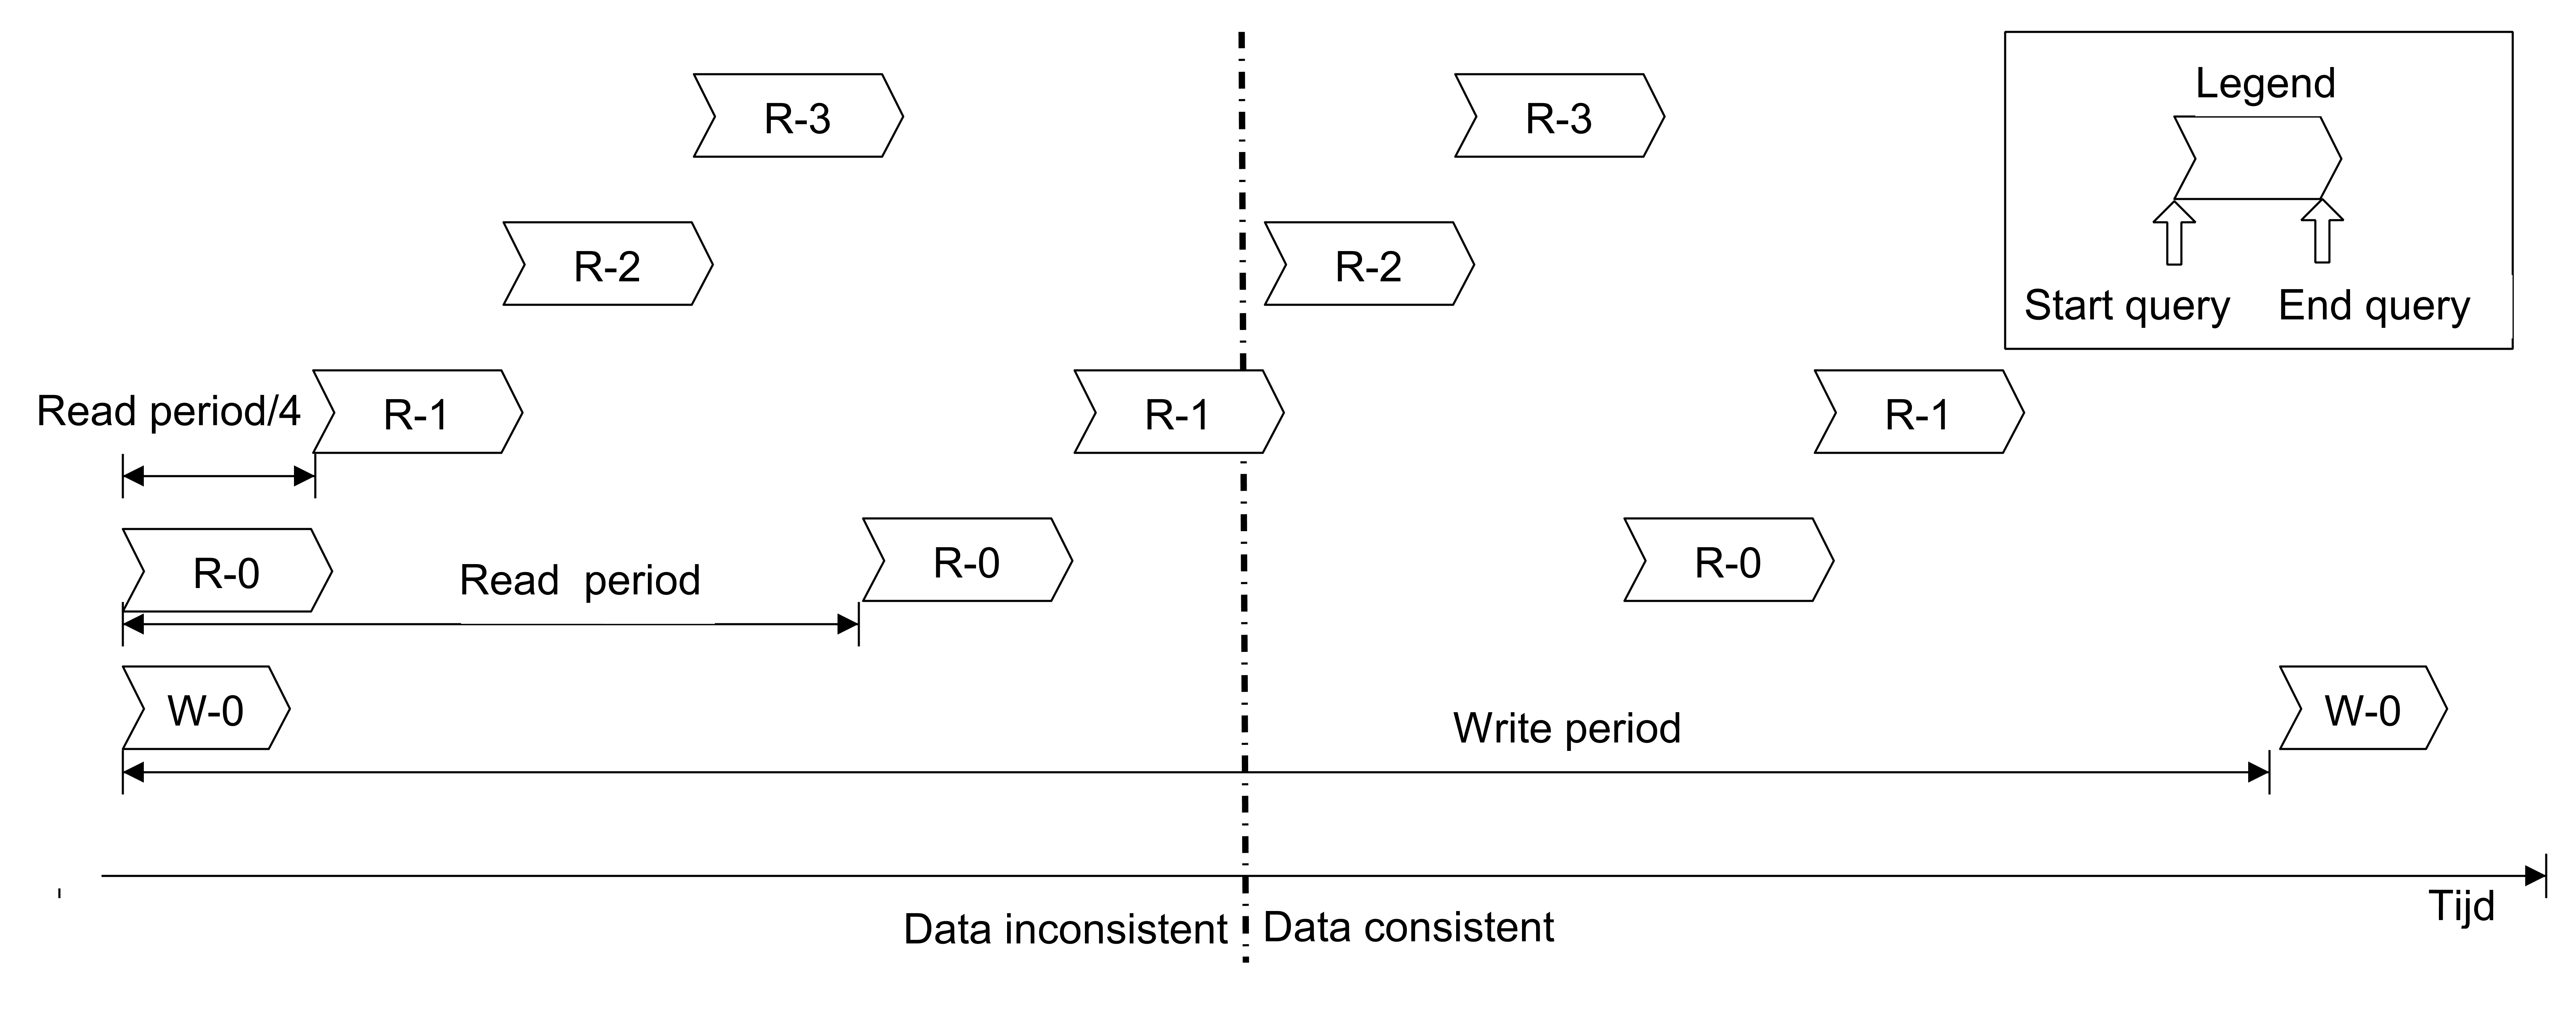
\includegraphics[width=\linewidth]{../img/Consistency-test-period}
\caption{Example of consistency support for one write period with 1 writer and 4 readers}
\end{figure}
These workloads exists out of 1 writer and a user-defined amount of readers.  Each writer will inserts or updates a value in the database with a user-defined period between them. The readers will read the record till they read the last written data element, each reader reads in a period defined by the user. The different readers are scheduled uniformly between the reading period. 

All this data is logged and gives possibilities to analyse when a record is visible for different users, compared to the time the queries where started or ended. 

Before the test are 30 000 records stored in the database and each tests takes 500 seconds and results start to be gathered after 30 seconds. In the tests is chosen to write every 0.5s and read with 5 readers every 10ms. 
 

\section{Results}\label{sec:result}
To execute the tests, both systems were deployed on a virtual platform of OpenStack. Each instance has 2 CPUs, 4GB RAM and 50GB disc space. The machines are connected with a gigabit Ethernet and an average ping takes 0.4ms ($\sigma = 0.2$ on 10 000 ping's).

HBase is configured with 7 instances, of which 3 for management (1 HMaster, Hadoop namenode and Zookeeper, and 2 extra Zookeeper instances) and 4 for data storage (each has a HRegionServer and Hadoop datanode). 

MongoDB is configured with 6 instance, grouped a 3 for a ReplicaSet. There was a single configuration server and 3 instances had an access server. 

YCSB was deployed on a single instance and used to calibrate the systems to have a basic workload. An individual record has 10 fields which each field a size of 100 bytes. The workload existed out of 20\% inserts and updates, 40\% selects and 20\% scans of an uniform spread between 1 and 100. The requests are spread according to Zipfian\footnote{Some record are popular, others rare to be used.}  The basic load for HBase is an average of 600 queries/second spread over 50 threads, for MongoDB there are 15 threads with a total of 200 queries/second. 

\subsection{Availability}
When reading and writing in the default setting of MongoDB, both MongoDB and HBase will read and write from a leader for a set of data. Both have a lease period for the leader, which can't be set for MongoDB (10 seconds), but can be configured for HBase (default 180 seconds). 

\begin{figure}[h]
\centering
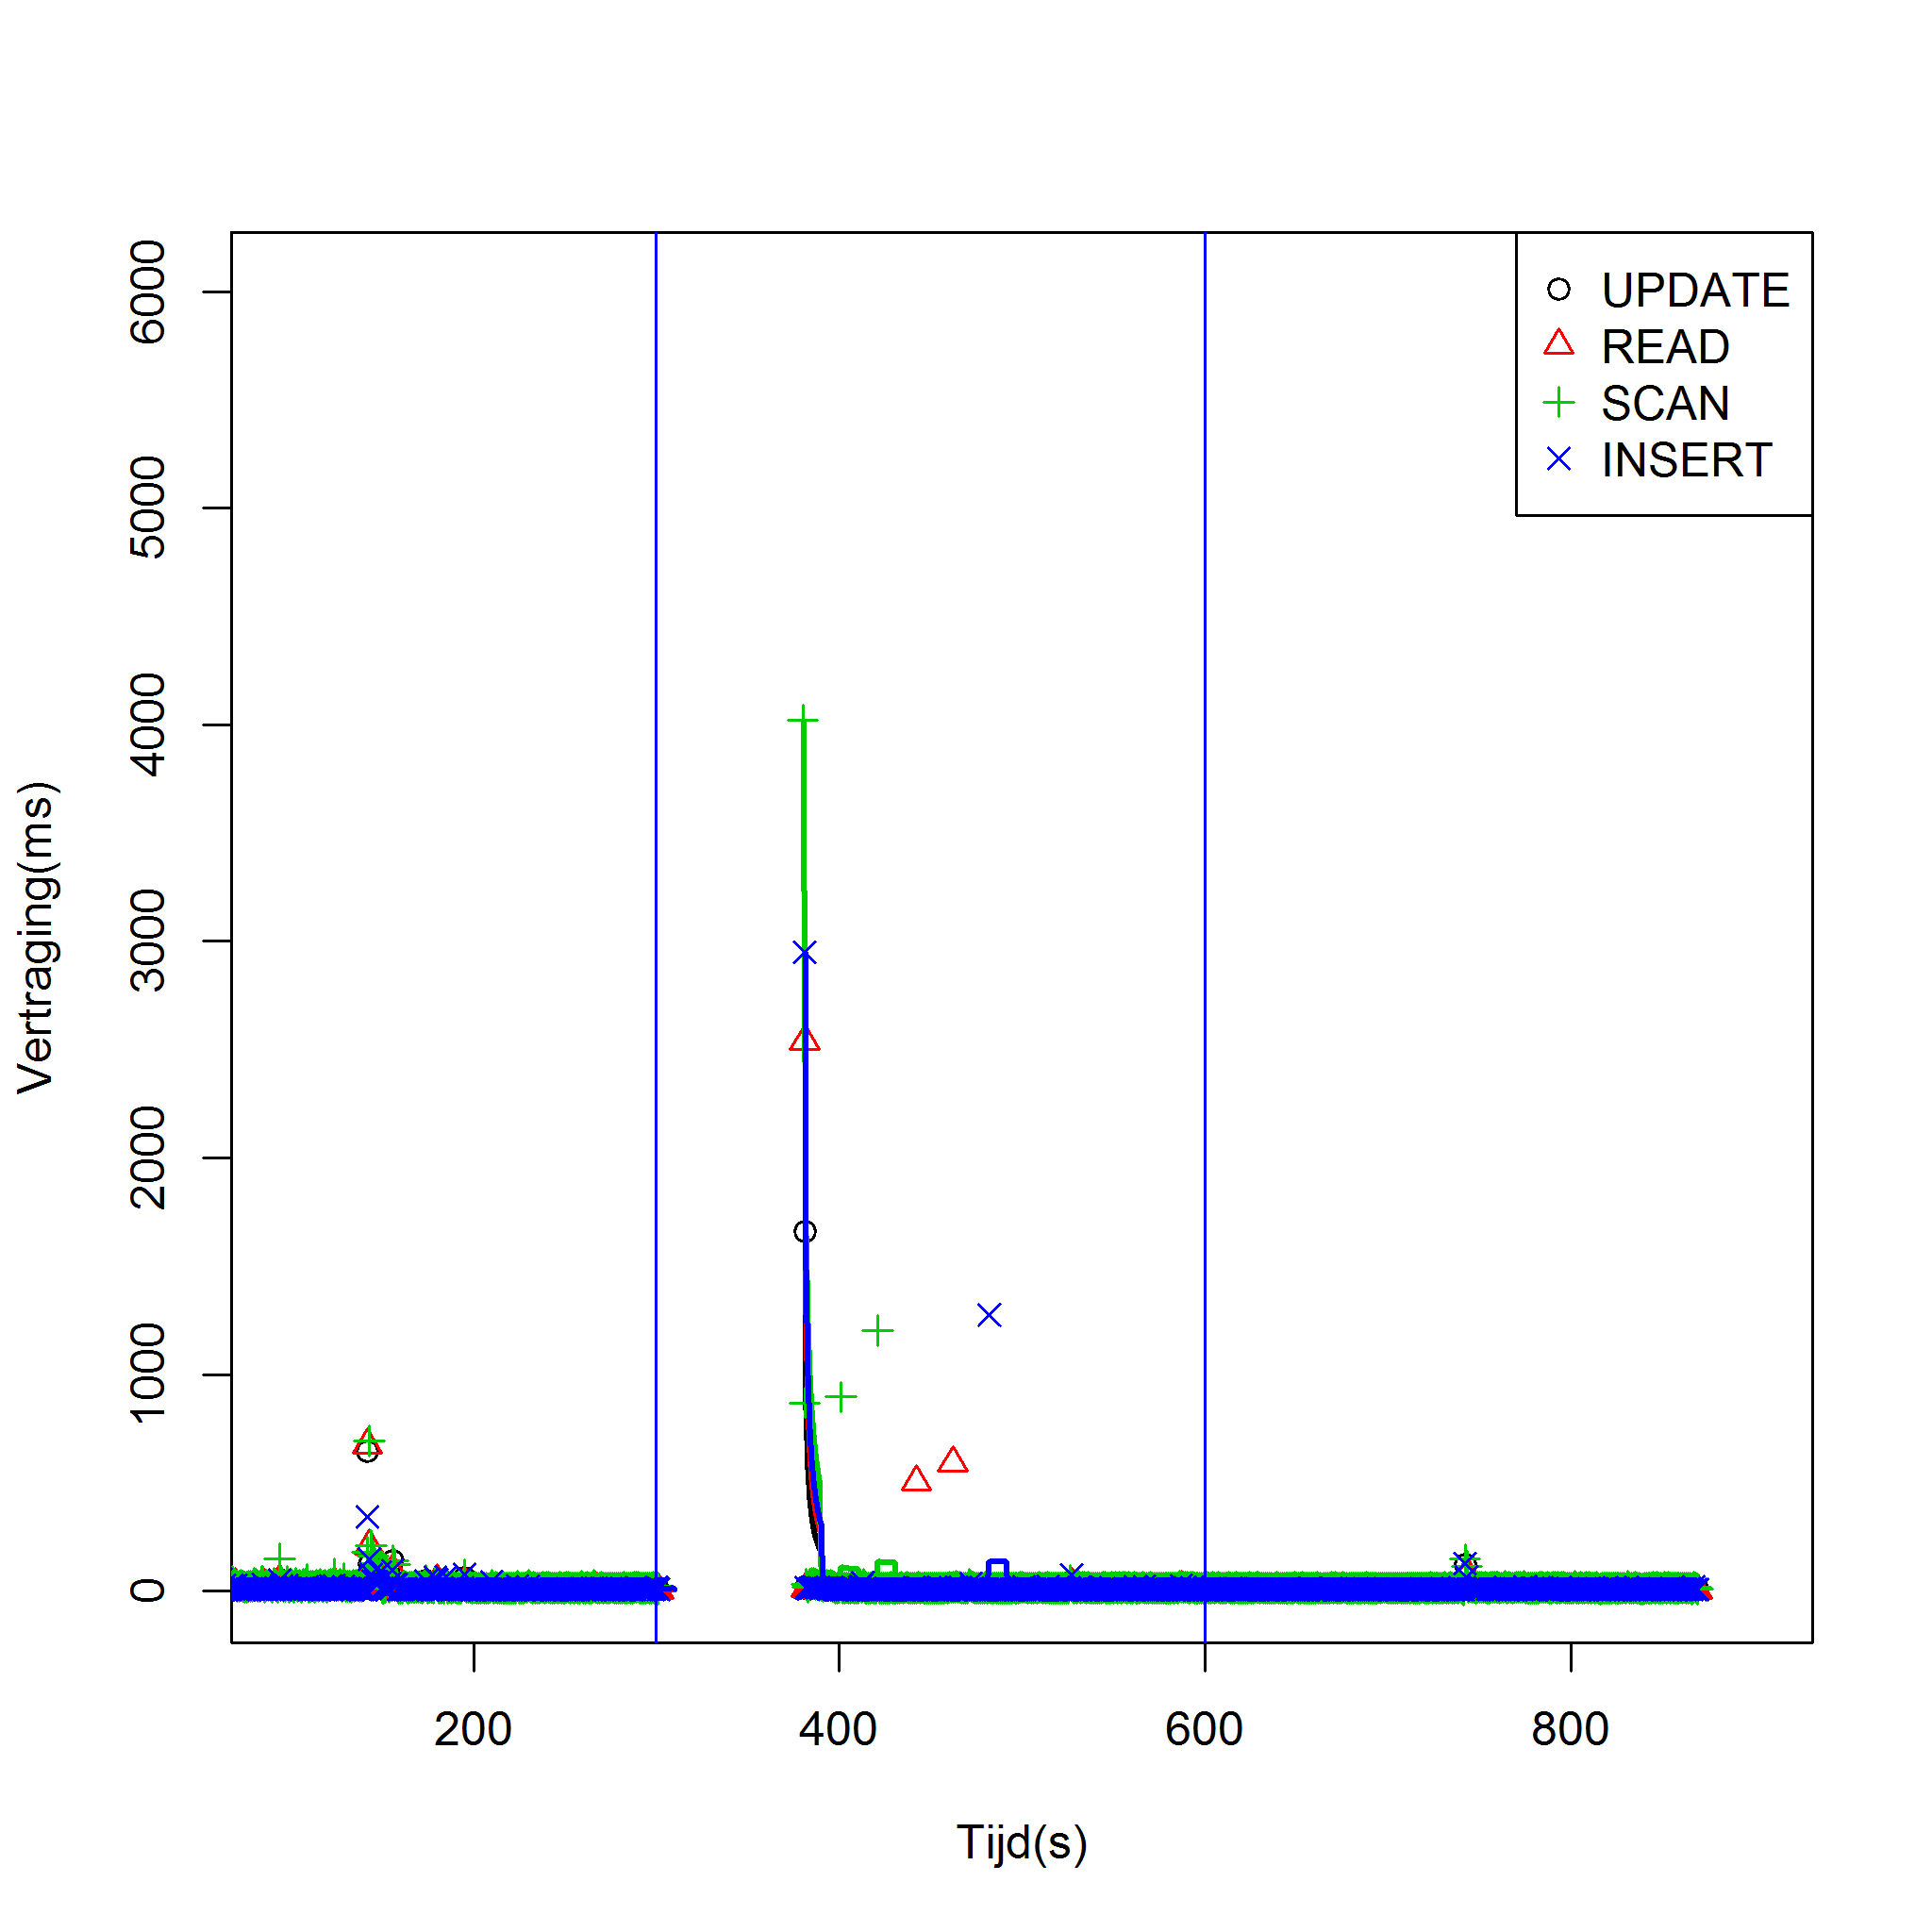
\includegraphics[width=\linewidth]{../img/Observaties/HBase/Stop-07-14-Soft-3-1.png}
\caption{Example of gracefullyl shutting down a HBase node. The requests block for 90 seconds }
\end{figure}

In case of a stop of a HBase server in this configuration, the queries will halt till the lease for the region has been expired, this can take between 0 seconds and 180, depending on the moment of the action. Normally a release is possible in a graceful shut down, but as the pictures shows, this doesn't happen always. 

For MongoDB, there is no difference between the graceful or hard stop of an instance; in case it was a secondary, no influences on the latency will be seen. In case a primary was stopped, will in both cases the data be temporarily unavailable.  In case of a network interruption, \todo{....}


\subsection{Consistency}
In consistency HBase and MongoDB have a different approach, more specific MongoDB has multiple configuration parameters for reading and writing while in H than HBase. 

\section{Future work}\label{sec:futurework}

\section{Related work}\label{sec:related work}
The research towards database systems and their consistency guaranties is rare to have a measured approach. In recent paper (February 2014), Golab et al. states that there is only a limited amount of research done towards eventual consistency \cite{golab2014eventually}. They present a new view on consistency, were already some research is done towards active analyse (how long before the data is replicated to all nodes), the amount of passive analyse is limited (what do the users see). Compared to the consistency results from this paper, both are discussed: as well the delays before the data is present everywhere but also on the acting of the specific systems, in example the behaviour of HBase. 

Another extension of YCSB called YCSB++\cite{patil2011ycsb++}, provides more logging information on all systems in the first place, but they also test the consistency of HBase in regards of the client caches. The reasoning for this is that it is the standard run configuration of HBase, but the submitting of the client cache towards the system depends not only on the time, but also on the amount of traffic that is being submitted. In the study they compare different cache sizes and this shows already a difference in time. Furthermore, it is possible to disable this caching in case there are records in the need of this strict consistency. 

For availability benchmarking, there was no research found on related databases. However, research from 2004 \cite{mauro2004system} discuss a way to let a standalone system recover and provide a starting benchmark for it.  


\section{Conclusion}\label{sec:conclusion}\todo{}

%% The Appendices part is started with the command \appendix;
%% appendix sections are then done as normal sections
%% \appendix

%% \section{}
%% \label{}

%% References
%%
%% Following citation commands can be used in the body text:
%% Usage of \cite is as follows:
%%   \cite{key}         ==>>  [#]
%%   \cite[chap. 2]{key} ==>> [#, chap. 2]
%%

%% References with bibTeX database:

\bibliographystyle{elsarticle-num}
\bibliography{referenties}
%% Authors are advised to submit their bibtex database files. They are
%% requested to list a bibtex style file in the manuscript if they do
%% not want to use elsarticle-num.bst.

%% References without bibTeX database:

% \begin{thebibliography}{00}

%% \bibitem must have the following form:
%%   \bibitem{key}...
%%

% \bibitem{}

% \end{thebibliography}


\end{document}

%%
%% End of file `elsarticle-template-num.tex'.
